\begin{figure}[h]
  \centering
  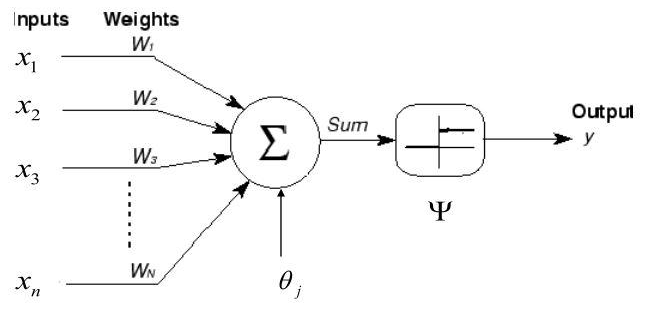
\includegraphics[width=11cm]{./Chapitre2/figures/perceptron.png}
  \caption{Représentation schématique d'un perceptron. $x_i$ correspond aux entrées, les $W_i$ correspondent aux poids associés à chacune des entrées $x_i$, $\psi$ formalise le biais. Une fois sommée, la valeur est passée dans une fonction d'activation $\phi$ pour déterminer la valeur de sortie $y$. Dans le schéma la fonction d'activation correspond à un simple signal échelon.}
  \label{fig:perceptron}
\end{figure}
